% Mettre un "%" devant les styles � ne pas utiliser
\documentclass{gig} % style Master GIG

\usepackage[latin1]{inputenc} 
\usepackage[frenchb]{babel} 
\usepackage{t1enc,dfadobe}
\usepackage{cite}

% for including postscript figures
% mind: package option 'draft' will replace PS figure by a filename within a frame
\ifpdf \usepackage[pdftex]{graphicx} \pdfcompresslevel=9
\else \usepackage[dvips]{graphicx} \fi


\title[Analyse de la g�om�trie d'un objet discret]{Analyse de la g�om�trie d'un objet discret dans un espace tri-dimensionnel}

\author[Laure Hatoufet et Laurent Larelu]%
       {Laure Hatoufet$^1$
        et Laurent Larelu$^{1,2}$
        \\
         $^1$Aix-Marseille Universit�\\
         $^2$Aix-Marseille Universit�
       }

\begin{document}

\maketitle

\begin{abstract}
   Ceci est un r�sum�.
\end{abstract}

\keywords{Mod�lisation g�om�trique, maillages, mot 3, mot 4.}

%-------------------------------------------------------------------------


\section{Introduction}

Contexte, probl�matique.

Lorem ipsum dolor sit amet, consectetur adipiscing elit, sed do eiusmod tempor incididunt ut labore et dolore magna aliqua. Ut enim ad minim veniam, quis nostrud exercitation ullamco laboris nisi ut aliquip ex ea commodo consequat. Duis aute irure dolor in reprehenderit in voluptate velit esse cillum dolore eu fugiat nulla pariatur. Excepteur sint occaecat cupidatat non proident, sunt in culpa qui officia deserunt mollit anim id est laborum \cite{REFIG1}. Lorem ipsum dolor sit amet, consectetur adipiscing elit, sed do eiusmod tempor incididunt ut labore et dolore magna aliqua. Ut enim ad minim veniam, quis nostrud exercitation ullamco laboris nisi ut aliquip ex ea commodo consequat. Duis aute irure dolor in reprehenderit in voluptate velit esse cillum dolore eu fugiat nulla pariatur. Excepteur sint occaecat cupidatat non proident, sunt in culpa qui officia deserunt mollit anim id est laborum.


\section{Travaux relatifs}

Ce qui se fait d'habitude dans le domaine, bref �tat de l'art, expos� rapide des m�thodes existantes.

Lorem ipsum dolor sit amet, consectetur adipiscing elit, sed do eiusmod tempor incididunt ut labore et dolore magna aliqua. Ut enim ad minim veniam, quis nostrud exercitation ullamco laboris nisi ut aliquip ex ea commodo consequat. Duis aute irure dolor in reprehenderit in voluptate velit esse cillum dolore eu fugiat nulla pariatur. Excepteur sint occaecat cupidatat non proident, sunt in culpa qui officia deserunt mollit anim id est laborum.

\subsection{Figures en couleur}

Il n'y a aucune censure � avoir sur les figures en couleur (voir figure \ref{fig:ex3}). 

\begin{figure*}[htb]
  \centering
  \mbox{} \hfill
  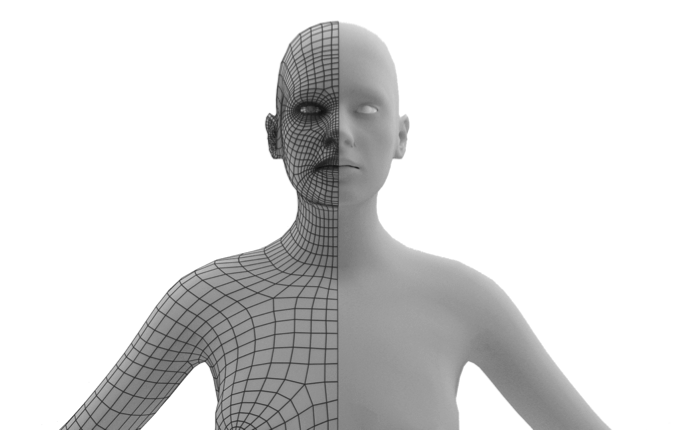
\includegraphics[width=.3\linewidth]{logoGIG}
  \hfill
  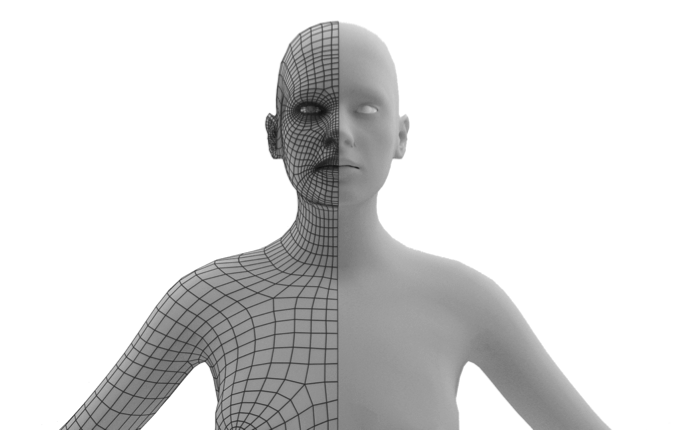
\includegraphics[width=.3\linewidth]{logoGIG}
  \hfill \mbox{}
  \caption{\label{fig:ex3}Les figures en couleurs ou en noir et blanc peuvent �tre plac�es n'importe o� dans le document. Elles peuvent �tre mises sur les 2 colonnes gr�ce � "figure*".}
\end{figure*}


\section{Expos� de la m�thode}

Votre m�thode, avec un sch�ma global qui explique les diff�rentes �tapes.

Algorithmes en pseudo-code.

R�partition des t�ches.

Lorem ipsum dolor sit amet, consectetur adipiscing elit, sed do eiusmod tempor incididunt ut labore et dolore magna aliqua. Ut enim ad minim veniam, quis nostrud exercitation ullamco laboris nisi ut aliquip ex ea commodo consequat. Duis aute irure dolor in reprehenderit in voluptate velit esse cillum dolore eu fugiat nulla pariatur. Excepteur sint occaecat cupidatat non proident, sunt in culpa qui officia deserunt mollit anim id est laborum.

\subsection{Tableau}

\begin{table}[h]
\centering
\begin{tabular}{|l|c|r|}
\hline
Laboratoire & Ville & Conf�rence\\ \hline\hline
 XLIM & Limoges & AFIG \cite{AFIG13} \\ \hline
& Laval & AFRV \cite{AFRV13}\\ \hline
LIAFA et LIGM & Paris & G�oDis \cite{GEODIS13}\\ \hline
\end{tabular}
\label{tab:tab1}
\caption{Exemple de tableau.}
\end{table}

\subsection{Equation}

\begin{equation}
x' + y^{2} = z_{i}^{2} \label{eq:eq1}
\end{equation}

L'�quation \ref{eq:eq1} n'est qu'un exemple d'�quation.

\begin{figure}[htb]
  \centering
  \mbox{} \hfill
  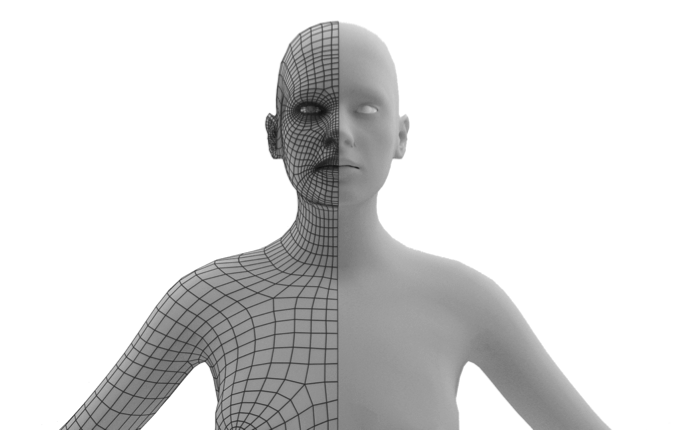
\includegraphics[width=\linewidth]{logoGIG}
  \hfill \mbox{}
  \caption{\label{fig:ex4} Une figure sur une seule colonne.}
\end{figure}


\section{R�sultats et validation}

R�sultats obtenus, difficult�s rencontr�es, les cas qui posent probl�me, discussion sur la m�thode.

Lorem ipsum dolor sit amet, consectetur adipiscing elit, sed do eiusmod tempor incididunt ut labore et dolore magna aliqua. Ut enim ad minim veniam, quis nostrud exercitation ullamco laboris nisi ut aliquip ex ea commodo consequat. Duis aute irure dolor in reprehenderit in voluptate velit esse cillum dolore eu fugiat nulla pariatur. Excepteur sint occaecat cupidatat non proident, sunt in culpa qui officia deserunt mollit anim id est laborum.

\section{Conclusion}

Conclusion, ce qui marche et ce qui marche moins bien.

Perspectives et travaux futurs : comment am�liorer l'approche dans le futur.

Lorem ipsum dolor sit amet, consectetur adipiscing elit, sed do eiusmod tempor incididunt ut labore et dolore magna aliqua. Ut enim ad minim veniam, quis nostrud exercitation ullamco laboris nisi ut aliquip ex ea commodo consequat. Duis aute irure dolor in reprehenderit in voluptate velit esse cillum dolore eu fugiat nulla pariatur. Excepteur sint occaecat cupidatat non proident, sunt in culpa qui officia deserunt mollit anim id est laborum.

%-------------------------------------------------------------------------
\newpage
\bibliographystyle{refig-alpha}
\bibliography{bibsample}
%-------------------------------------------------------------------------




\end{document}
